\clearpage\begingroup
\providecommand{\InstrumentMoneyMark}{%
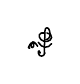
\begin{tikzpicture}[x=.024em,y=-.024em,baseline=-.72em,line width=.055em,line cap=round,line join=round]
\path[use as bounding box] (0,0) rectangle (37,43);
\draw (25,39) .. controls (25,28) and (26,12) .. (26,5)
 .. controls (26,-2) and (32,-1) .. (33,5)
 .. controls (35,12) and (33,17) .. (28,18);
\draw (26,8) .. controls (17,6) and (15,13) .. (20,18)
 .. controls (25,23) and (35,21) .. (36,15)
 .. controls (37,11) and (33,8) .. (29,8);
\draw (16,22) .. controls (21,31) and (31,32) .. (36,24);
\draw (26,38) .. controls (25,44) and (17,45) .. (16,38)
 .. controls (15,34) and (19,34) .. (19,38);
\draw (15,28) .. controls (12,23) and (8,19) .. (6,23)
 .. controls (3,28) and (7,33) .. (9,28)
 .. controls (10,22) and (5,21) .. (3,26)
 .. controls (0,29) and (1,32) .. (3,31);
\end{tikzpicture}}

\SourceLeaf{299}\NoSourceHead
\begin{center}{\Large [BERICHTE UND ANTRÄGE\par
ZUR ANSCHAFFUNG VON INSTRUMENTEN\par
FÜR DIE GÖTTINGER STERNWARTE.]}\par\medskip
\rule{.80\textwidth}{.35pt}\par
{\small [Aus den Akten des Kuratoriums der Universität Göttingen.]}\par
\rule{.80\textwidth}{.35pt}\par\medskip
[I.]\end{center}
\noindent\hspace*{\parindent}Unterthänigstes P[ro] M[emoria]\\
die Anschaffung der Instrumente für die\\
neue Sternwarte in Göttingen betreffend.

Da der Bau des Hauptgebäudes der neuen Sternwarte im Wesentlichen jetzt so gut wie vollendet ist, und nach dem Beschluss des hohen königl. Curatorium der Bau der Seitenflügel im nächsten Frühjahr mit Nachdruck betrieben werden wird, so rückt nun die gänzliche Vollendung dieses für die Universität und für die Wissenschaft selbst gleich wichtigen Instituts immer näher. Schon zwölf Jahre sind seit seiner ersten Gründung verflossen. Es ist gewiss, dass die Erwartung des ganzen für die Astronomie sich interessirenden Europa auf die künftige Thätigkeit desselben gerichtet ist. Es ist höchst wünschenswerth, dass diese Thätigkeit sofort nach Vollendung des Baues auf eine würdige Art anfangen könne: allein dazu ist unumgänglich nöthig, dass die Sternwarte im Besitz von wenigstens einem der erst herbeizuschaffenden Hauptinstrumente sei.

Der ganzen Anlage der neuen Sternwarte, in Rücksicht der Instrumente, wofür sie eingerichtet ist, liegt ein \textls[120]{ganz bestimmter Plan} zum Grunde, bei welchem sowohl auf die bereits vorhandenen, als auf die demnächst aus
\clearpage\SourceLeaf{300}\HistoricalHead{295}{R}{BERICHTE UND ANTRÄGE ZUR ANSCHAFFUNG VON INSTRUMENTEN.}
\noindent Lilienthal zu erwartenden, als endlich auf die neu anzuschaffenden [Instrumente] ganz bestimmte Rücksicht genommen ist. Da die Hauptinstrumente besonders unter den letztern eine äusserst feste Aufstellung erfordern, so ist für jedes derselben gleich zu Anfang ein besonderes 12 Fuss tiefes Fundament aus festen Quadern gelegt. Freilich hat in dem beträchtlichen seitdem verflossenen Zeitraume die Instrumentalastronomie in mehrern Stücken wichtige Verbesserungen und Abänderungen erhalten, die auch bei jenem Plane einige Modificationen nöthig machen werden: inzwischen werden doch jene Fundamente im Wesentlichen ihre ursprüngliche Bestimmung behalten.

Um nun beurtheilen zu können, was von den neu anzuschaffenden Instrumenten zuerst und am dringendsten nöthig sein wird, muss wenigstens eine allgemeine Uebersicht der Bedürfnisse einer Sternwarte vom ersten Range, wie die hiesige werden soll, vorausgehen, wobei ich jedoch alles weitläuftige Detail vermeiden will.

Die Hauptbedürfnisse einer Sternwarte nach dem heutigen Zustande der praktischen Astronomie lassen sich auf drei Classen zurückführen, Uhren, Sehwerkzeuge und Messwerkzeuge; letztere zerfallen wiederum in bewegliche und feste. Was ausser diesen Rubriken etwa noch erforderlich ist, wie z. B. Barometer, Thermometer und dergl., sind verhältnissmässig nur Kleinigkeiten, bei welchen ich mich hier nicht aufhalten will.

\textls[120]{Uhren.} Die Anzahl der auf einer Sternwarte nothwendigen astronomischen Uhren hängt von der Ausdehnung des Locals ab. Auf einer Sternwarte wie die hiesige alte, welche nur aus Einem Saale besteht, war Eine Hauptuhr hinreichend; auf der neuen Sternwarte werden drei erforderlich sein, nämlich eine in der westlichen Abtheilung, die zweite in der östlichen, die dritte in der Rotunde. Zu diesen drei Pendeluhren muss noch eine tragbare Uhr (Chronometer) hinzukommen, um jene unter sich vergleichen zu können.

Ein freilich nur französischer, aber zu diesem Zweck hinreichend guter Chronometer ist bereits vorhanden; auch ist die Hauptpendeluhr der alten Sternwarte von \textsc{Shelton}, obgleich sie schon über 40 Jahre daselbst im Gange ist, noch immer sehr gut, und vollkommen werth, auf der neuen Sternwarte eine der drei Hauptuhren zu werden. Die alte Sternwarte hat zwar ausser derselben noch ein Paar andere Pendeluhren, die indessen nur wenig Werth haben, und hier also nicht in Betracht kommen. Zwei Pendeluhren von der
\clearpage\SourceLeaf{301}\HistoricalHead{296}{L}{PRAKTISCHE UND SPHÄRISCHE ASTRONOMIE.}
\noindent ersten Güte müssen demnach noch hinzukommen. Zu den allerdringendsten Bedürfnissen gehören indessen dieselben nicht. In der Rotunde ist nicht eher eine Uhr nöthig, als bis das dahin zu setzende Aequatorealinstrument zugleich da ist, so wie in den beiden Abtheilungen der untern Sternwarte die Uhren zugleich mit den daselbst aufzustellenden Instrumenten da sein müssen. Ueberdies hat die Sternwarte in Zukunft aus Lilienthal auch eine Pendeluhr zu erwarten, die wie ich glaube als eine von den Hauptuhren wird dienen können.

\textls[120]{Sehwerkzeuge} d. i. achromatische Fernröhre und Spiegelteleskope. Die alte Sternwarte besitzt von Instrumenten dieser Classe mehrere recht gute; noch weit mehr wird sie aber in Zukunft aus Lilienthal erhalten, wo sich bekanntlich ein grosser Reichthum von Spiegelteleskopen, zum Theil von grossen Dimensionen, befindet. In dieser Beziehung bleibt demnach wenig zu wünschen übrig.

\textls[120]{Bewegliche Messinstrumente.} Aus dieser Classe besass die alte Sternwarte vor noch nicht langer Zeit nur wenig, was auf der neuen einen Platz verdient hätte. Allein durch verschiedene seit drei Jahren aus München von dem berühmten Künstler \textsc{Reichenbach} erhaltene Instrumente nemlich\par
\noindent\hspace*{\parindent}einen 12zolligen \textsc{Borda}ischen Kreis\\
\hspace*{\parindent}einen\enspace 8zolligen Theodolith und\\
\hspace*{\parindent}einen $3\frac12$fussigen Heliometer, zu welchem ich das im vorigen Jahre bestellte parallatische Stativ täglich erwarte, ist diese Lücke schon grossentheils ausgefüllt, so dass nur hauptsächlich noch ein guter Spiegelkreis zu wünschen ist, wie sie der englische Künstler \textsc{Troughton} u. a. verfertigen. Dies Instrument ist indessen theils kein sehr grosses Objekt, theils gehört dessen Anschaffung auch nicht zu den dringendsten Bedürfnissen, indem die Sternwarte einen freilich nur sehr schlecht gearbeiteten Spiegelkreis von einem französischen Künstler besitzt, der wenn auch unbrauchbar zu wirklichen Beobachtungen, doch dazu dienen kann, beim Unterricht die Einrichtung dieses Instruments zu zeigen, welches besonders bei der Schifffahrt so wichtig ist.

Bei allen bisher betrachteten Rubriken fanden wir demnach kein sehr dringendes Bedürfniss; allein anders verhält es sich mit den\par
\noindent\hspace*{\parindent}\textls[120]{Festen Messinstrumenten}, welche fast alle erst neu anzuschaffen sind. Von diesen wird daher etwas umständlicher gehandelt werden müssen.
\clearpage\SourceLeaf{302}\HistoricalHead{297}{R}{BERICHTE UND ANTRÄGE ZUR ANSCHAFFUNG VON INSTRUMENTEN.}
Dem von Anfang an entworfenen Plane zufolge soll die neue Sternwarte folgende fünf feste Instrumente enthalten, für welche schon im Voraus alle Einrichtungen berechnet und getroffen sind.\par
\noindent\hspace*{\parindent}A. Ein Aequatoreal, in der Rotunde aufzustellen, wofür das Drehdach eingerichtet ist.\par
\noindent\hspace*{\parindent}B. Ein grosses Passageinstrument, unten, in der westlichen Abtheilung.\par
\noindent\hspace*{\parindent}C. Ein grosser Meridiankreis, ebendaselbst.\par
\noindent\hspace*{\parindent}D. Ein kleineres Passageinstrument, in der östlichen Abtheilung.\par
\noindent\hspace*{\parindent}E. Der schon auf der alten Sternwarte seit 60 Jahren befindliche Mauerquadrant ebendaselbst.

Für die Instrumente B, C, D, E sind die oben erwähnten Fundamente gelegt und die beiden Durchschnitte des Gebäudes sowie die Dachklappen eingerichtet.

Es wird nöthig sein, von diesen Instrumenten wenigstens mit einigen Zügen den Gebrauch zu bezeichnen.

Als Hauptzweck aller grossen Sternwarten in wissenschaftlicher Rücksicht muss angesehen werden »die Bewegungen und Stellungen der Himmelskörper auf der Himmelskugel mit der höchsten Präcision zu bestimmen«. Diese Stellungen werden bestimmt durch die sogenannten geraden Aufsteigungen, gerade eben so wie die Oerter auf der Erde durch Breite und Länge bestimmt werden. Am zweckmässigsten ist es, diese Bestimmungen immer dann zu machen, wo die Himmelskörper eben in der Mittagsfläche sich befinden oder wo sie, wie man es nennt, culminiren. Und gerade dies ist die Bestimmung der Instrumente B, C, D, E; die Passageinstrumente B, D dienen für die geraden Aufsteigungen; der Meridiankreis C dient für die Abstände vom Pol, zu welchem Zweck man ehemals den Mauerquadranten E anwandte, der aber nach der neuern Beobachtungsart dazu bei weitem nicht so zweckmässig ist, als der Meridiankreis.

Es gibt aber Fälle, wo die Beobachtung eines Himmelskörpers im Augenblick der Culmination unmöglich ist; dann ist man gezwungen, ihn ausser der Mittagsfläche zu beobachten, und dazu dient das Aequatoreal A, und zwar für gerade Aufsteigung und Abstand vom Pol zugleich. Das Aequatoreal ist also gewissermassen ein Nothbehelf, wo die Meridianinstrumente nicht ausreichen.
\HistoricalFoot{XI 1.}{38}
\clearpage\SourceLeaf{303}\HistoricalHead{298}{L}{PRAKTISCHE UND SPHÄRISCHE ASTRONOMIE.}
Aus dieser kurzen Darstellung geht schon hervor, dass die Instrumente B, C als die wichtigsten der ganzen Sternwarte angesehen werden müssen. Diese, wenn sie von der ersten Güte sind, erheben eigentlich die Sternwarte zum ersten Range, und die Beobachtungsregister, welche von den ersten Sternwarten z. B. der Greenwicher jährlich gedruckt werden, enthalten fast gar nicht anderes als die täglichen, mit den Meridianinstrumenten angestellten Beobachtungen, und auf diesen seit 50 oder 60 Jahren gedruckten Greenwicher Beobachtungen beruhet der grösste Theil der heutigen Astronomie. Nicht eher wird sich die Göttinger Sternwarte neben die Greenwicher, Pariser, Mayländer, Palermer und die eben jetzt zur Vollendung kommenden Ofner und Neapler Sternwarten stellen können, als bis sie mit tüchtigen Meridianinstrumenten versehen ist.

Uebrigens muss ich noch bemerken, dass dem Plane nach die Instrumente D, E hauptsächlich für den Unterricht bestimmt sein sollen, oder für solche weniger wichtige Beobachtungen, um derentwillen man etwa Beobachtungen an den Hauptinstrumenten B, C nicht stören oder unterbrechen will. Soll aber der Mauerquadrant, welcher nur ein schlechtes, nichtachromatisches Fernrohr hat (er wurde noch vor Erfindung der achromatischen Fernröhre verfertigt), und an dem mehrere Haupttheile durch den langen Gebrauch sich sehr ausgeschliffen haben, diesen Dienst wirklich leisten können, so muss er ein ganz neues achromatisches Fernrohr, neue Zapfenbewegung u. s. f. bekommen.

Es ergibt sich hieraus, dass, wenn die neue Sternwarte nach gänzlicher Vollendung des Baues nicht noch lange feiern soll, die beiden Hauptinstrumente B und C wenigstens nun bald bestellt werden müssen, zumal da man bei solchen grössern Instrumenten immer mehrere Jahre warten muss. Hiebei muss nun aber noch ein wichtiger Umstand in Betracht gezogen werden.

Der Bestellung des Passageinstruments B stände an sich nichts im Wege und das Beste wäre, dies bei dem berühmten und einzigen Künstler \textsc{Reichenbach} zu thun. Diese Instrumente haben im Wesentlichen jetzt eine sehr bestimmte Einrichtung und nur die Vollkommenheit der Ausführung unterscheidet eines von dem andern. Allein anders verhält es sich mit den Meridiankreisen. Die Instrumente welche diesen Namen führen sind zum Theil von ganz
\clearpage\SourceLeaf{304}\HistoricalHead{299}{R}{BERICHTE UND ANTRÄGE ZUR ANSCHAFFUNG VON INSTRUMENTEN.}
\noindent verschiedner Einrichtung und noch ist es nicht ganz entschieden, welcher der höchste Preis gebührt.

Der erste Meridiankreis, welcher in der praktischen Astronomie eine Epoche gemacht hat, war der, welchen die Palermer Sternwarte vor einigen 20 Jahren von dem berühmten \textsc{Ramsden} erhielt, und bei dem Plane zu unserer neuen Sternwarte hat man ohne Zweifel einen solchen im Sinn gehabt. Dieser Kreis kostete damals etwas über 3000 Thaler; seine Grösse ist 5 Fuss im Durchmesser.

Vor etwa 10 oder 12 Jahren vollendete ein ungemein geschickter Künstler in Hamburg, \textsc{Repsold}, einen Meridiankreis, beinahe 4 Fuss im Durchmesser, von einer ganz verschiedenen und sehr sinnreichen Einrichtung, der auch das Eigenthümliche hat, dass er zugleich das Passageinstrument in sich vereinigt. Dies Instrument, von welchem nachher noch weiter die Rede sein wird, ist eine Reihe von Jahren hindurch in einer kleinen auf dem Hamburger Walle erbauten Sternwarte (die aber in der neuesten Zeit abgetragen wurde) aufgestellt gewesen, und manche vortreffliche Beobachtungen sowohl von dem Künstler selbst, als von Hrn. \textsc{Schumacher}, jetzigem Director der Mannheimer Sternwarte, damit angestellt.

Eine noch viel grössere Celebrität haben aber die seit wenigen Jahren von \textsc{Reichenbach} verfertigten 3fussigen Meridiankreise erworben, welche wiederum eine gänzlich verschiedene Einrichtung haben, und an Genauigkeit alles, was bis dahin geleistet war, übertreffen. Auf vielen der berühmtesten Sternwarten hat man sich beeifert, solche Kreise (deren Preis ehemals gegen 2000 \InstrumentMoneyMark\ war, neuerlich aber wie ich höre bedeutend erhöhet ist) anzuschaffen; der Künstler hat dergleichen für Mayland, Marseille, Ofen, Paris, Neapel, München verfertigt.

So höchst vortrefflich nun diese \textsc{Reichenbach}schen dreifüssigen Kreise auch sind, so scheint es doch fast, als ob ein neuer sechsfussiger Kreis von dem englischen Künstler \textsc{Troughton}, der seit ein Paar Jahren in Greenwich aufgestellt ist, sie noch übertrifft. Dieser Kreis, den man zum Unterschiede einen Mauerkreis nennt, hat abermals eine ganz andere Einrichtung: aber einer Privatnachricht zufolge soll er 1800 Guinees gekostet haben. Nach ganz neuerlich erhaltenen Nachrichten soll auch \textsc{Reichenbach} wieder auf wichtige
\HistoricalFoot{}{$38^{\ast}$}
\clearpage\SourceLeaf{305}\HistoricalHead{300}{L}{PRAKTISCHE UND SPHÄRISCHE ASTRONOMIE.}
\noindent Abänderungen und Verbesserungen bei seinen Kreisen bedacht gewesen sein, die ihnen vielleicht wieder den entschiedenen Vorrang geben werden.

Da es bei dem Verhältnisse, in welchem das Königreich Hannover zu England steht, wohl nicht für unmöglich angesehen werden muss, dass trotz des hohen Preises eines solchen Mauerkreises auch die Göttinger Sternwarte noch einen solchen Vorzug etwa durch eine ausserordentliche Munificenz des Prinzen Regenten erhalten könnte, und da auf alle Fälle im gegenwärtigen Augenblick die allervortheilhafteste Einrichtung der Meridiankreise noch immer streitig ist, so wäre \textls[120]{von dieser Seite} betrachtet am rathsamsten, den Entschluss hierüber und die Bestellung noch etwas zu verschieben, während von der andern Seite es doch höchst wichtig ist, dass die neue Sternwarte gleich nach der Vollendung auf eine würdige Art in Thätigkeit komme. Man könnte freilich das Passageinstrument B sogleich bestellen, allein mit diesem allein können nur unvollständige Beobachtungen gemacht werden, und die Sternwarte würde noch ganz der Selbstständigkeit ermangeln.

Unter diesen Umständen muss ein Ausweg willkommen sein, wodurch alle Wünsche sich vereinigen lassen, und wodurch ausserdem noch die Möglichkeit gewonnen wird, die Kosten für die neu anzuschaffenden Instrumente auf mehrere Jahre füglicher zu vertheilen. Dieser Ausweg besteht darin, sofort den oben erwähnten \textsc{Repsold}schen Kreis anzuschaffen, den, wie ich jetzt bestimmt weiss, der Künstler für 1300—1400 Thaler (Hamburgisch) abzulassen erbötig ist, mehrere daran zu machende Abänderungen, welche ich wünschte, mit inbegriffen.

Mein Plan ist nicht, dass dies Instrument noch ausser den 5 oben angeführten Instrumenten hinzukommen soll; auf diese Art würde selbst kein Platz dafür da sein. Sondern es sollte dafür das kleinere Passageinstrument D ganz wegfallen, und auf demselben Platze, wohin dieses bestimmt war, jener Kreis aufgestellt werden. Nach den Versicherungen des Baumeisters \textsc{Müller} könnte das Zimmer, wohin dieser Kreis also kommen würde, mit leichter Mühe ganz ausgebaut und so schon gegen den nächsten Herbst das Instrument aufgestellt und gebraucht werden.

Der Vortheil hievon wäre nun sehr evident. Der \textsc{Repsold}sche Kreis wird freilich den neuesten \textsc{Reichenbach}schen und \textsc{Troughton}schen Kreisen an Vollkommenheit nachstehen; allein aus eigner Ansicht des Instruments, aus
\clearpage\SourceLeaf{306}\HistoricalHead{301}{R}{BERICHTE UND ANTRÄGE ZUR ANSCHAFFUNG VON INSTRUMENTEN.}
\noindent Berichten mehrerer meiner astronomischen Freunde\textsuperscript{*)}, endlich aus der Prüfung vieler damit gemachten Beobachtungen habe ich die Ueberzeugung, dass dies Instrument, welches Kreis und Passageinstrument in sich vereinigt, ein sehr vortreffliches ist, welches sich füglich dazu qualificirt, solange auf der neuen Sternwarte als Hauptinstrument zu dienen, bis die Instrumente B und C herbeigeschafft sind.
\begingroup\renewcommand{\thefootnote}{*)}\footnotetext{Herr v. \textsc{Lindenau}, der das Instrument später als ich gesehen hat, nachdem ein neues Fernrohr von 8 Fuss Länge daran angebracht war, versicherte, dies Fernrohr gehöre zu den vollkommensten die er kenne, und stehe dem 8fussigen Fernrohr am Passageinstrument der Seeberger Sternwarte (von \textsc{Ramsden}) nicht nach.}\endgroup

Die neue Sternwarte wird demnach schon 2 oder 3 Jahre früher als sonst möglich wäre, eine würdige Thätigkeit beginnen können, womit sie schon einen sehr ehrenvollen Platz unter den ersten Sternwarten erhält. Es wird nun weniger dringend, die Instrumente B und C sogleich zu bestellen, was besonders in Rücksicht auf C ein grosser Vortheil ist; auch B mag dann immerhin ein Jahr später bestellt werden, als sonst nöthig wäre, obwohl doch gut wäre, nicht gar zu lange damit zu warten.

Auf zwei Einwürfe habe ich noch zu antworten:\par
\noindent\hspace*{\parindent}I. Die Vergrösserung der Kosten betreffend, so ist dieselbe, näher betrachtet, so gut wie gar keine. Das kleine Passageinstrument D, welches nun wegfällt, würde wenigstens 700 Thaler und die oben erwähnten Reparaturen am Mauerquadranten, \textls[120]{welche dann auch wegfallen könnten}, würden auch circa 600 \InstrumentMoneyMark\ betragen. Der Mauerquadrant sollte zu einem doppelten oben angegebenen Zweck dienen; zum Unterricht ist er auch ohne die Reparaturen eben so brauchbar, für eigentliche Beobachtungen von wissenschaftlichem Werth wird er durch den \textsc{Repsold}schen Kreis ersetzt, der doch ohne Vergleich mehr leistet, als der Mauerquadrant selbst nach allen Reparaturen leisten könnte. Sollten also die Kosten auf diese Weise auch noch eine Kleinigkeit mehr betragen als nach dem ursprünglichen Plane der Fall gewesen sein würde, so wird dies mehr als compensirt, durch den Vortheil, gerade die grössten Ausgaben für Instrumente noch ein und mehrere Jahre weiter hinausschieben zu können.\par
\noindent\hspace*{\parindent}II. In Beziehung auf den Unterricht ist das Wegfallen des kleinen Passageinstrumentes, wenn an dessen Stelle der \textsc{Repsold}sche Kreis tritt,
\clearpage\SourceLeaf{307}\HistoricalHead{302}{L}{PRAKTISCHE UND SPHÄRISCHE ASTRONOMIE.}
\noindent durchaus kein Verlust, sondern wahrer Gewinn. Das kleinere Passageinstrument D zeigte doch nur im Kleinen, was B im Grossen zeigt, und die Zöglinge der praktischen Astronomie erhalten nun Gelegenheit, noch ein Instrument mehr von einer ganz originellen Einrichtung kennen zu lernen. Dass das wichtige Instrument B dabei keiner Gefahr ausgesetzt werde, muss der Direktor verhüten und kann es nach meinen Erfahrungen auch; ganz ungeschickten Händen würde man auch das Instrument D nicht haben Preis geben dürfen.

Das Fundament für D ist glücklicherweise so, dass es mit geringen Abänderungen auch für den \textsc{Repsold}schen Kreis benutzt werden kann.

Noch ein wichtiger Umstand verdient bemerkt zu werden. Ich weiss, dass ein gewisser anderer auswärtiger Astronom gleichfalls Absichten auf dies Instrument hat. Ich habe mich vorher bei Hrn. \textsc{Repsold} versichert, dass es jetzt noch uns zu Gebote steht. Ob dies aber nach einigen Monaten noch der Fall sein würde, wage ich nicht zu verbürgen.

Nach allen hier aufgeführten Gründen, unterwerfe ich es nun dem höhern Ermessen des königl. hohen Curatorium, ob mein hier gethaner Vorschlag Dessen Genehmigung verdiene, und sehe den weitern Verfügungen in tiefster Ehrfurcht entgegen.

Göttingen den 9. Februar 1815.
\begin{flushright}C. F. \textsc{Gauss}.\end{flushright}
\clearpage\endgroup
